\section{可编程逻辑器件典型工艺}

\subsection{反熔丝技术}
\begin{frame}[allowframebreaks]{反熔丝技术}

\begin{block}{\textbf{起源与发展}:}
\begin{itemize}
\tightlist
\item
该项目由美国斯坦福大学发明。
\item
第一种开发出来的用户可编程开关是 \textbf{熔丝},广泛应用于可编程逻辑阵列(PLA)中。
\item
由 \textbf{Actel} 公司开发,该公司后被 \textbf{Microsemi} 公司收购,而 \textbf{Microsemi} 公司又被 \textbf{Microchip} 公司收购。
\end{itemize}
\end{block}
\pagebreak
\begin{center}
    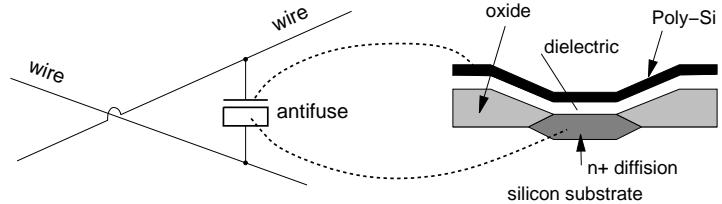
\includegraphics[width=0.8\textwidth, height=0.6\textheight, keepaspectratio]{img1/antifuse.jpeg}\\
    反熔丝技术示意图
\end{center}

\begin{block}{\textbf{反熔丝基础特性}:}
\begin{itemize}
\tightlist
\item
在初始状态下是开路的。
\item
只有在编程后才会呈现低电阻特性。
\item
适用于FPGA,可通过改进的CMOS技术实现。
\end{itemize}
\end{block}
\pagebreak
\begin{block}{\textbf{技术实现}:}
\begin{itemize}
\tightlist
\item
    \textbf{PLICE结构}(由Actel公司开发)\footnote<.->[frame]{E. Hamdy et
    al, ``Dielectric-based antifuse for logic and memory ICs,'' IEEE
    International Electron Devices Meeting Technical Digest, pp.~786 -
    789, 1988.} :

    \begin{itemize}
    \tightlist
    \item
    位于两条互连导线之间。
    \item
    由三层结构组成:

    \begin{itemize}
    \tightlist
    \item
        顶层和底层为导体(多晶硅和n+扩散层)。
    \item
        中间层为绝缘体(ONO,氧化物-氮化物-氧化物)。
    \end{itemize}
    \item
    未编程状态:绝缘体隔离顶层和底层。
    \item
    编程状态:绝缘体转变为低电阻连接。
    \end{itemize}
\item
    \textbf{其他反熔丝结构}\footnote<.->[frame]{J. Birkner et al, ``A
    very-high-speed field-programmable gate array using metal-tometal
    antifuse programmable elements,'' Microelectronics Journal, v. 23,
    pp.~561-568}:

    \begin{itemize}
    \tightlist
    \item
    采用金属作为导体。
    \item
    中间层为非晶硅。
    \end{itemize}
\end{itemize}
\end{block}
\end{frame}

\begin{frame}[allowframebreaks]{PLICE反熔丝的特性与应用}
\phantomsection\label{pliceux53cdux7194ux4e1dux7684ux7279ux6027ux4e0eux5e94ux7528}
\begin{itemize}
\tightlist
\item
    \textbf{尺寸与电气性能优势}:

    \begin{itemize}
    \tightlist
    \item
    反熔丝足够小,可以适应通道布线轨迹的宽度,\textbf{PLICE}
    反熔丝在尺寸和电气性能方面具有关键优势。
    \item
    这意味着反熔丝本身基本上不会产生芯片尺寸开销。
    \end{itemize}
\item
    \textbf{架构突破}:

    \begin{itemize}
    \tightlist
    \item
    \textbf{PLICE} 反熔丝的小尺寸和低延迟特性,使得 \textbf{Actel}
    在以下两个关键架构上取得突破:

    \begin{itemize}
    \tightlist
    \item
        提供丰富的布线资源,同时保持非常小的芯片尺寸。
    \item
        提供高度灵活、高度精细的架构(如小的逻辑块)。
    \end{itemize}
    \end{itemize}
    \pagebreak
\item
    \textbf{一次性编程特性}:

    \begin{itemize}
    \tightlist
    \item
    采用这种工艺的可编程逻辑器件(PLD)一旦编程后,其内部连接关系将永久固化,无法再修改。
    \item
    由于是一次性器件,一旦编程失败或设计出现缺陷,整个器件将报废,必须重新采购新的器件。
    \item
    这导致设计成本较高。
    \end{itemize}
\item
    \textbf{抗干扰与保密性能}:

    \begin{itemize}
    \tightlist
    \item
    采用这种工艺的 PLD 具有优异的抗干扰性能和保密性能。
    \item
    由于整个设计已经被固化到芯片内,破解芯片内的设计结构异常困难。
    \end{itemize}
\end{itemize}
\end{frame}

\subsection{PROM、EPROM和EEPROM工艺}
\begin{frame}[allowframebreaks]{PROM、EPROM和EEPROM工艺}
\textbf{可编程只读存储器}(\textbf{Programmable Read Only
Memory},\textbf{PROM})是一种可编程逻辑器件。

\textbf{PROM} 内部由固定的逻辑与阵列和可编程的逻辑或阵列构成。

当使用 \textbf{PROM} 时,可以通过最小项求和的方式实现布尔逻辑函数功能

\begin{figure}
\centering
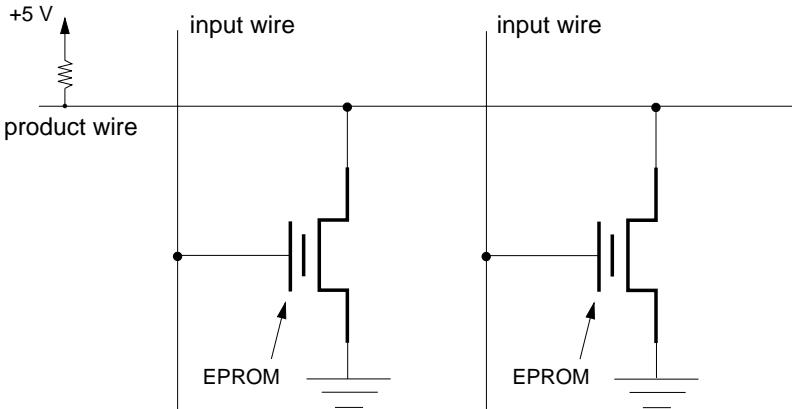
\includegraphics[width=0.7\textwidth]{img1/EPROM.jpeg}
\caption{EPROM可编程开关结构图}
\end{figure}

\begin{itemize}
\tightlist
\item
    浮栅晶体管类似于 EPROM 和 EEPROM 中使用的晶体管。
\item
    在 CPLD 中,浮栅晶体管被用作可编程开关,并广泛应用于许多 SPLD 中。
\item
    实现方式:

    \begin{itemize}
    \tightlist
    \item
    将晶体管放置在两条导线之间,以便实现线与(wired-AND)功能。
    \item
    示例:

    \begin{itemize}
    \tightlist
    \item
        图3展示了 EPROM 晶体管在 CPLD 的与门平面中的连接方式。
    \item
        如果某个输入是相应乘积项的一部分,则该输入可以通过 EPROM
        晶体管将与产品线驱逻辑电平``0''。
    \item
        对于不参与乘积项的输入,相应的 EPROM 晶体管被编程为永久关闭。
    \end{itemize}
    \end{itemize}
\item
    EEPROM 器件的工作方式与此类似。
\end{itemize}
\end{frame}

\subsection{SRAM可编程开关}
\begin{frame}[allowframebreaks]{SRAM的技术特点}
\textbf{Xilinx} 公司(被 \textbf{AMD} 公司收购)和 \textbf{Altera}
公司(被 \textbf{Intel} 公司收购)的绝大多数 \textbf{FPGA} 采用
\textbf{SRAM} 工艺。
\begin{figure}
    \centering
    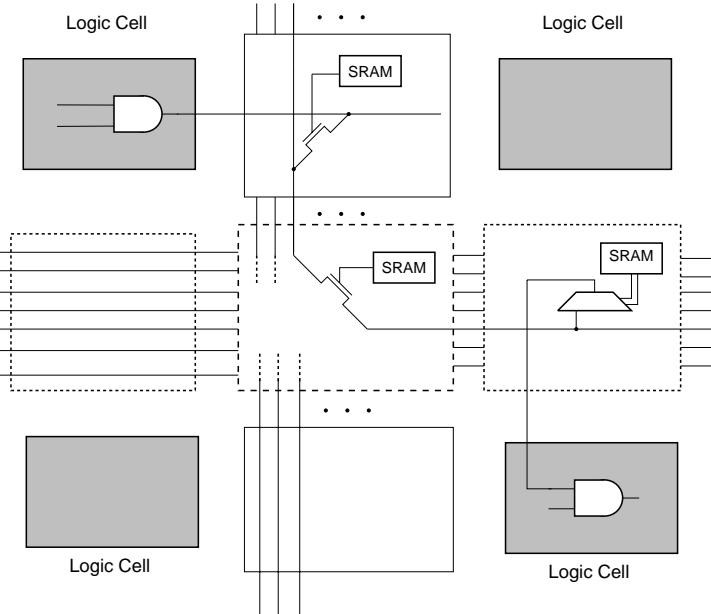
\includegraphics[width=0.4\textwidth]{img1/SRAM.jpeg}
    \caption{SRAM可编程开关}
\end{figure}

\begin{itemize}
\tightlist
\item
    \textbf{SRAM 和反熔丝}:

    \begin{itemize}
    \tightlist
    \item
    尽管 EPROM 或 EEPROM 技术理论上也适用于 FPGA,但目前商用 FPGA
    产品主要基于 SRAM 或反熔丝技术。
    \end{itemize}
\item
    \textbf{SRAM 单元的应用}:

    \begin{itemize}
    \tightlist
    \item
    用于控制传输晶体管(pass-transistor)开关的栅极节点。
    \item
    用于控制多路复用器(multiplexer)的选择线,从而驱动逻辑块输入。
    \end{itemize}
\end{itemize}


\begin{itemize}
\tightlist
\item
    \textbf{示例连接}:

    \begin{itemize}
    \tightlist
    \item
    图5展示了一个逻辑块(由左上角的与门表示)通过两个传输晶体管开关和一个多路复用器连接到另一个逻辑块的过程。
    \item
    所有这些开关和多路复用器都由 SRAM 单元控制。
    \end{itemize}
\item
    \textbf{FPGA 的实现方式}:

    \begin{itemize}
    \tightlist
    \item
    FPGA
    是否使用传输晶体管、多路复用器或两者结合,取决于具体产品的设计。
    \end{itemize}
\item
    只读存储器(Read Only
    Memory,ROM)采用掩膜工艺,它属于非易失性存储器。
\item
    当系统断电后,信息仍然保留在 ROM 内的存储单元中。

    \begin{itemize}
    \tightlist
    \item
    用户可以从掩膜器件中读取信息,但是不能往 ROM 中写入任何信息。
    \item
    ROM 单元保存了行和列数据,形成一个阵列,每一列有负载电阻使其保持逻辑
    1,每个行列的交叉有一个关联晶体管和一个掩膜连接。
    \end{itemize}
\end{itemize}
\end{frame}

\begin{frame}{SRAM在FPGA中的应用}
在采用 SRAM 工艺的 FPGA 中,SRAM 单元主要实现以下三个任务,包括:

\begin{itemize}
\tightlist
\item
    作为查找表(Look-Up Table,LUT)实现逻辑(用作真值表)。
\item
    用作嵌入式块存储器资源(比如缓冲区存储)。
\item
    用于控制布线和配置开关。
\end{itemize}
\end{frame}

\begin{frame}{SRAM工艺的优缺点}
\begin{itemize}
\tightlist
\item
    采用这种工艺的 PLD 优势主要体现在:

    \begin{itemize}
    \tightlist
    \item
    易于修改(甚至可以动态可重配置)。

    \begin{itemize}
    \tightlist
    \item
        设计者可以对 PLD 进行反复修改和编程。
    \end{itemize}
    \item
    较好的密度。
    \item
    跟踪最新的 SRAM 技术(比逻辑技术更快)。
    \item
    灵活,实现结构更好。

    \begin{itemize}
    \tightlist
    \item
        不但适用于有限自动状态机,同时也适用于算术电路。
    \end{itemize}
    \end{itemize}
\item
    采用这种工艺的 PLD 的劣势在于:

    \begin{itemize}
    \tightlist
    \item
    采用这种工艺的 PLD 属于易失性器件。

    \begin{itemize}
    \tightlist
    \item
        只要系统正常供电,器件配置信息就不会丢失;一旦断电,保存在 FPGA
        内的配置信息将丢失。
    \item
        在使用 SRAM 工艺的 FPGA 进行数字系统设计时,需要在 FPGA
        的外部连接一个存储器芯片来保存器件配置信息的原因。
    \end{itemize}
    \item
    通常具有较大的功耗。
    \end{itemize}
\end{itemize}
\end{frame}

\begin{frame}
\begin{block}{SRAM编程技术总结}
\phantomsection\label{sramux7f16ux7a0bux6280ux672fux603bux7ed3}
\begin{itemize}
\tightlist
\item
    \textbf{存储机制}:6晶体管单元存储配置位\\
\item
    \textbf{技术特征}:

    \begin{itemize}
    \tightlist
    \item
    支持无限次擦写(\textgreater10\^{}15次)\\
    \item
    静态功耗约0.5μW/bit\\
    \item
    与标准CMOS工艺兼容\\
    \end{itemize}
\item
    \textbf{缺点}:

    \begin{itemize}
    \tightlist
    \item
    存储数据需要消耗大量的硅片面积,且断电后数据信息丢失。
    \end{itemize}
\end{itemize}
\end{block}
\end{frame}


\subsection{flash工艺}
\begin{frame}[allowframebreaks]{flash器件结构}

\begin{figure}
    \centering
    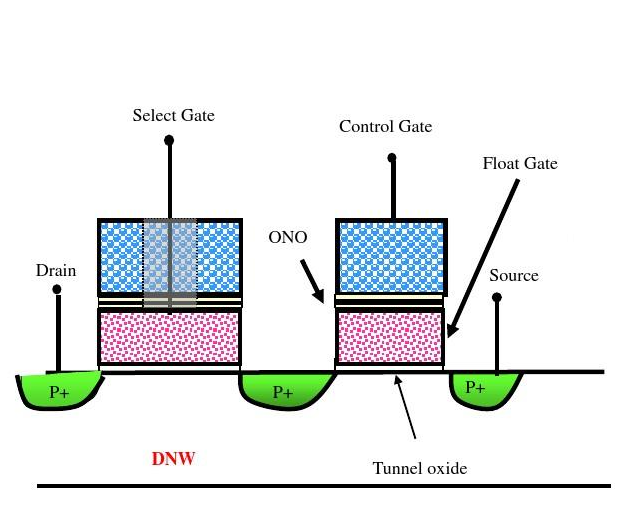
\includegraphics[width=0.5\textwidth]{img1/flash.png}
    \caption{flash器件结构图}
\end{figure}

\begin{itemize}
\tightlist
\item
    真正的基于FLASH工艺的FPGA不应与内部带有FLASH存储器的FPGA类型混淆。\\
\item
    具有内部FLASH存储器的基于SRAM的FPGA仅在启动期间使用FLASH存储器将数据加载到SRAM配置单元。\\
\item
    真正基于FLASH工艺的FPGA使用FLASH作为配置存储的主要资源,并且不需要SRAM。\\
\item
    功耗低。\\
\item
    对辐射效应更宽容。
\end{itemize}
\end{frame}

\begin{frame}{采用FLASH工艺的PLD}
\begin{itemize}
\tightlist
\item
    \textbf{特性}:

    \begin{itemize}
    \tightlist
    \item
    具有多次可重复编程的能力。\\
    \item
    非易失性:断电后,器件配置信息仍保存在PLD内。
    \end{itemize}
\item
    \textbf{结构}:

    \begin{itemize}
    \tightlist
    \item
    FLASH可采用多种结构,与EPROM单元类似,具有一个浮置栅晶体管单元和EEPROM器件的薄氧化层特性。
    \end{itemize}
\end{itemize}
\end{frame}

\begin{frame}{Flash编程技术总结}
\phantomsection\label{flashux7f16ux7a0bux6280ux672fux603bux7ed3}
\begin{itemize}
\tightlist
\item
    \textbf{存储机制}:

    \begin{itemize}
    \tightlist
    \item
    浮栅晶体管电荷存储
    \end{itemize}
\item
    \textbf{技术特征}:

    \begin{itemize}
    \tightlist
    \item
    非易失性存储\\
    \item
    单元密度较SRAM提升40\%\\
    \item
    耐受$10^4$~$10^5$次编程周期
    \end{itemize}
\end{itemize}
\end{frame}

\subsection{可编程逻辑器件工艺总结}
\begin{frame}{可编程逻辑器件工艺总结}
    \begin{table}[h!]
    \centering
    % \scriptsize
    \begin{tabular}{|l|c|c|c|}
    \hline
    \textbf{工艺类型} & \textbf{可重复编程} & \textbf{易失性} & \textbf{技术} \\ \hline
    熔丝 (Fuse) & 否 & 否 & 双极型 \\ \hline
    EPROM & 是(需移出电路) & 否 & UVCMOS \\ \hline
    EEPROM & 是(可在电路内) & 否 & EECMOS \\ \hline
    SRAM & 是(可在电路内) & 是 & CMOS \\ \hline
    反熔丝 (Antifuse) & 否 & 否 & CMOS+ \\ \hline
    \end{tabular}
    \end{table}
\end{frame}